\documentclass[a4paper]{article}

%\usepackage{mathptmx}
%\usepackage{amsmath}
\usepackage[english]{babel}
\usepackage{subcaption}
\usepackage[width=.8\textwidth]{caption}
\usepackage{float}
\usepackage{hyperref}
\usepackage[utf8]{inputenc}
\usepackage{multicol}
\usepackage{longtable}
\usepackage{minted}
\usepackage{xargs}
\usepackage[pdftex,dvipsnames,table,xcdraw]{xcolor}
\usepackage{pdfpages}
\usepackage{booktabs}
\usepackage{multirow}
\usepackage{rotating,tabularx}
\usepackage{tabularx,ragged2e}
\newcolumntype{L}{>{\RaggedRight\arraybackslash}X}
\usepackage[colorinlistoftodos,prependcaption,textsize=tiny]{todonotes}
\newcommandx{\unsure}[2][1=]{\todo[linecolor=red,backgroundcolor=red!25,bordercolor=red,#1]{#2}}
\setlength{\marginparwidth}{2cm}

\usepackage{titlesec}

\titlespacing*\section{0pt}{12pt plus 4pt minus 2pt}{0pt plus 2pt minus 2pt}
\titlespacing*\subsection{0pt}{12pt plus 4pt minus 2pt}{0pt plus 2pt minus 2pt}
\titlespacing*\subsubsection{0pt}{12pt plus 4pt minus 2pt}{0pt plus 2pt minus 2pt}

\begin{document}
\title{Knowledge and the Web \\ 
\large{Proposal to Detect Fallacies}}
\author{\textsc{Group 1: Pieter Delobelle, Murilo Cunha, Eric Massip}}
\date{\today}
\maketitle

\section{Research question}
The general research question is to detect fallacies, but given the large number of possible fallacies---both formal and informal---we choose to focus primarily on the \emph{ad hominem} fallacy. 

This topic is related to fake news through the media outlets. Debates and interviews are a large part of the contemporary media. But by allowing invalid arguments to broadcast to billions of people, incorrect beliefs can be formed. Since some invalid arguments slip through the cracks of the journalists, automatically detecting fallacies can be a step towards better, less fake news.

In addition to this, President Donald Trump has made the term \emph{fake news} in itself an \emph{ad hominem} insult towards news outlets as well. 

\section{Datasets}

\subsection{General fallacy dataset~\cite{Habernal.et.al.2017.EMNLP}}
\url{https://github.com/UKPLab/argotario/}

TU Darmstadt assembled a small dataset (~1300 sentences) of both English and German sentences, labeled with one of 5 fallacies or none. These fallacies are:

\begin{itemize}
    \item ad hominem
    \item appeal to emotion
    \item hasty generalization
    \item irrelevant authority
    \item red herring
\end{itemize}

Some of these, like \emph{irrelevant authority}, are more conceptually. Others, like \emph{ad hominem} or \emph{incomplete comparison} (not in dataset), are more formally defined. In conclusion, this dataset might be a good starting point, but lacks a lot of interesting fallacies. Also, the small size might be an obstacle later on, requiring us to label additional sentences, which can be challenging to do in a short timeframe. 

More specifically, for the \emph{ad hominem} case, there are 589 records of \emph{ad hominem} fallacies and non-fallacies. Out of those, 382 were manually selected as adequate for training data. 

\begin{sidewaystable}
    \caption{...}\label{table:general-dataset}
    \begin{tabularx}{\textwidth}{@{}LlLlll@{}}
    \hline
    fTopic                                  & Intended Fallacy & Text                                                                                                                        & Eric & Pieter & Murilo \\ \hline
    Are humans to blame for certain animal extinctions? & No Fallacy                    & Yes, human beings have hunted and eaten animals for as long as can be shown and they are partly to blame for certain animal extinctions. & 1    & 1      & 1      \\
    Are humans to blame for certain animal extinctions? & No Fallacy                    & Humans are not to be blamed for animal extinction.                                                                                       & 0    & 1      & 1      \\
    Are humans to blame for certain animal extinctions? & No Fallacy                    & OF course they are!                                                                                                                      & 0    & 0      & 0      \\
    Are humans to blame for certain animal extinctions? & No Fallacy                    & We know that only the fittest can survive in this world.                                                                                 & 0    & 0      & 0      \\
    Are humans to blame for certain animal extinctions? & No Fallacy                    & just a test arg                                                                                                                          & 0    & 0      & 0      \\
    Are humans to blame for certain animal extinctions? & No Fallacy                    & Yes, they are.                                                                                                                           & 0    & 0      & 0      \\
    Are humans to blame for certain animal extinctions? & Ad Hominem                    & Extinction is not natural, you dont know what you are talking about!                                                                     & 1    & 0      & 0      \\
    Are humans to blame for certain animal extinctions? & No Fallacy                    & Humans don't care enough for living beings.                                                                                              & 1    & 1      & 1      \\
    Are humans to blame for certain animal extinctions? & No Fallacy                    & Humans must be blamed for using animals.                                                                                                 & 0    & 0      & 0      \\ \hline
    \end{tabularx}
\end{sidewaystable}

\subsection{Ad hominem dataset~\cite{Habernal.et.al.2018.NAACL.adhominem}}
\url{https://github.com/UKPLab/naacl2018-before-name-calling-habernal-et-al}
This dataset is also assembled by TU Darmstadt, focussed on the likelihood of a discussion ending in an \emph{ad hominem} attack. The data was sourced from a Reddit community focused on discussions (Change My View) and labeled by multiple people.  

Aside form the dataset, the related article~\cite{Habernal.et.al.2018.NAACL.adhominem} might also be an excellent starting point for the analysis of the \emph{ad hominem} fallacy, even though it is focused on how controversial statements have a higher than average change to end in an \emph{ad hominem} attack.

In total, this dataset contains 29,278 paragraphs or comments, of which 3,866 are labeled as \emph{ad hominem}.


\section{Examples}

\begin{itemize}
    \item \emph{Your argument that I should stop stealing candy from the corner store is no good. You told me yourself just one week ago that you, too, stole candy when you were a kid.}\footnote{Borrowed from~\cite{Walton1998}, p. 18}.
    
    In this quote, the second sentence is an \emph{ad hominem} attack, because tries to paint the first arguer as hypocritical. 

    Some peculiar features in this sentence are the combination of the words `\emph{you}' and `\emph{too}', indicating the behavior or an action of the first speaker  that contradicts his claim. Also the sequence ``\emph{you told me yourself}'' seems to attack an earlier statement of the first speaker, perhaps even out of an entirely different context. Both are features on a word or n-gram level.

    The sequence ``\emph{your argument (\dots) is no good}'' does attack the argument instead of the first speaker, and later on an \emph{ad hominem} attack follows. So depending on the dataset, this sequence might be ubiquitous in the set of fallacies.
    
    \item \emph{You're literally just quoting half of the amendment and then insisting the language isn't ambiguous. Implying I don't understand the English language isn't a winning argument.}\footnote{Borrowed from~\cite{Habernal.et.al.2018.NAACL.adhominem}}.
    
    This is an example of quote which could potentially be classified as an \emph{ad hominem} attack.
    
    At the start of the quote, the contraction ``\emph{You're}`` indicates that the counter-argument is analyzing the other person's initial reasoning and not attacking his or her personality per se. In this case, we should use a method which took into account a vector of words like ``\emph{You're literally just quoting}'' so the classifier can have a broader understanding of the speaker's intentions.
    
    In the second sentence, \emph{understand the English language} is very likely to appear in an \emph{ad hominem} attack as diminishing the ability of the other person to understand English. 
    
\end{itemize}
 
\section{Intended model outcome}
The ideal model should---given our earlier requirements---be able to predict with a certain accuracy/confidence if a given sentence or paragraph contains an \emph{ad hominem} fallacy. The confidence of the model will depend on the accuracy we are able to achieve. 

Our model will not classify if the given quote contains a fallacy or not. It will classify if the given quote contains an \emph{ad hominem} type of fallacy or not.

The user would have to keep in mind that the length of the paragraph can affect the analysis of it, meaning that more words and the interplay of those words can confuse the classifier. Furthermore, more sentences establish a bigger context and that could affect where specific sentences are fallacious or not.

\begin{figure}
    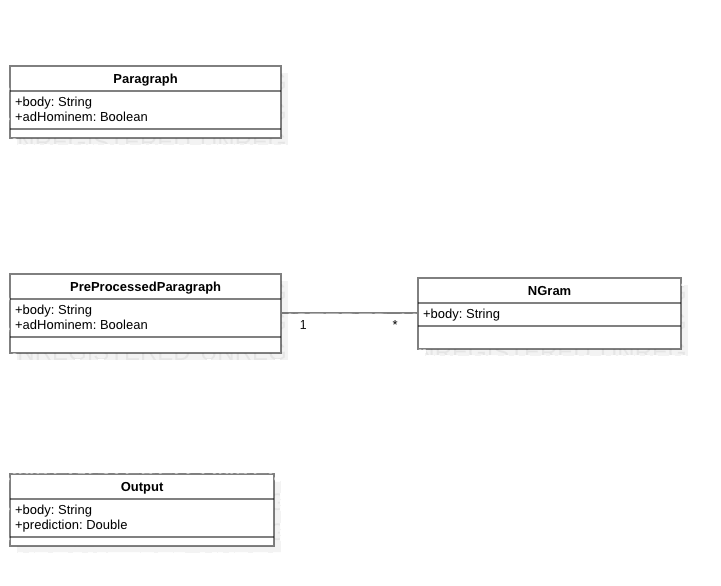
\includegraphics[width=1\textwidth]{figures/png/Model!Main_0.png}
    \caption{UML class diagram of training input, preprocessed input, and final output.}
    \label{fig:class-diagram}
\end{figure}

\begin{figure}
    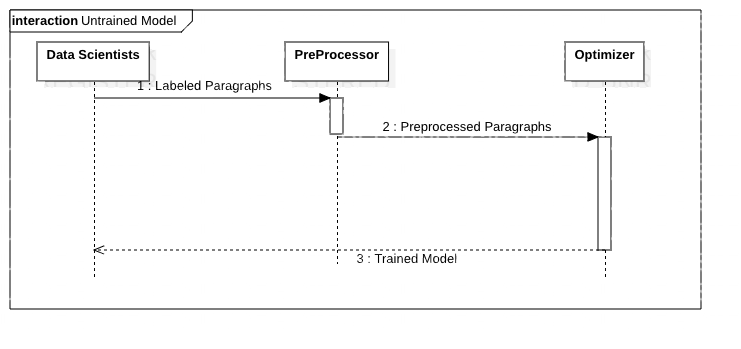
\includegraphics[width=1\textwidth]{figures/png/Collaboration2!Interaction1!UntrainedModel_2.png}
    \caption{UML sequence diagram of the untrained model.}
    \label{fig:untrained-diagram}
\end{figure}

\begin{figure}
    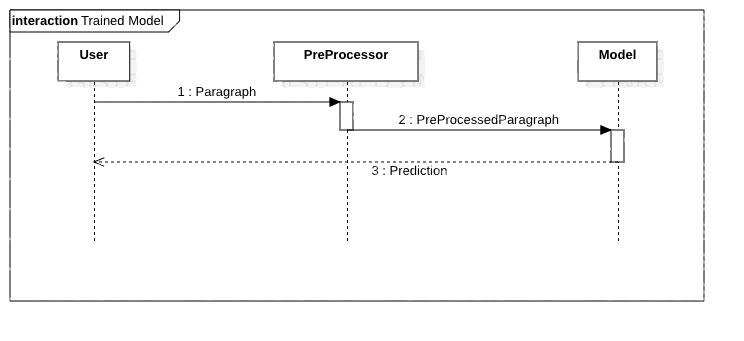
\includegraphics[width=1\textwidth]{figures/png/Collaboration1!Interaction1!TrainedModel_1.png}
    \caption{UML sequence diagram of the trained model.}
    \label{fig:trained-diagram}
\end{figure}

\section{Data schema}
Figure~\ref{fig:class-diagram} describes the classes input for the machine learning model. 

\begin{enumerate}
    \item \textbf{Paragraph}: Raw paragraph, either inserted by the user and thus unlabeled, or from a labeled dataset for training.
    \item \textbf{Preprocessed paragraph}: Same as the aforementioned \emph{Paragraph}, but with an added relation to a set of $N$-Grams. 
    \item \textbf{$N$-Gram}: Collection of subsets of $N$ words from the preprocessed paragraph. 
    \item \textbf{Output}: Output data containing the prediction as a numerical value, alongside the original paragraph.
\end{enumerate}

\section{Interaction overview}
The workflow for our model is split into two parts, depending on the goal. For training the model, the sequence diagram in Figure~\ref{fig:untrained-diagram} describes the basic approach and Figure~\ref{fig:trained-diagram} illustrates how an end user can call the trained model to make a classification---in the literature often called a prediction---on paragraphs provided by him or her. 


\bibliographystyle{IEEEtran}
\bibliography{main}

\end{document} 